\documentclass[../main/main.tex]{subfiles}

\newdate{date}{08}{10}{2020}


\begin{document}

\marginpar{ \textbf{Lecture 3.} \\  \displaydate{date}. \\ Compiled:  \today.}

\section{Basic models}

In this lecture we are going to introduce some of the basic models we will use for the entire course. The first assumption we make is that we are in \textbf{well-mixed populations}, or in other words \textit{homogeneous mixing}. Mathematically, it is what is called \textbf{mean field approximation}.

In the well-mixed population assumptions, it holds that that:
\begin{itemize}
\item all individuals are \textbf{equivalent}, hence every one has the same probability of being infected;
\item every individual has the \textbf{same number of contacts} $N-1$, or on average $\expval{k}$;
\item we are in a \textbf{closed population}. That is to say that the sum of the density distribution of the individuals is equal to 1, hence we have no deaths or births. In practice, we are assuming that our time scale is so little that we can consider the population constant.
\end{itemize}

\subsection{SI model}

The simplest model one can think of is the \textbf{SI} (\textbf{S}\textit{usceptible} \textbf{I}\textit{nfected}). In this model one can get the infection and, once we have got, we cannot recover, that is to say we stay infected forever.

The \textbf{transition diagram} that describes this model is the following:
\begin{equation}
  S + I \overset{\beta }{\rightarrow} I + I
\end{equation}
where $\beta$ is the \textit{“per contact” infection rate} and dictates the speed of the spreading. We can write down the \textbf{equation} that can be solved exactly:
\begin{equation}
\begin{split}
  \dv{s}{t} &= - \beta \expval{k} s i \\ \dv{i}{t} &= \beta \expval{k} s i
\end{split}
\end{equation}
where $\expval{k}$ represents the average contacts, while $i$ stands for the fraction of infected people in the entire population ($i=I/N$), and $s$ is the fraction of susceptible people in the population ($s=S/N$). Note as prefactor $\expval{k}$ is constant, therefore sometimes it can be "absorbed" inside $\beta$. 
The product $s i$ is the probability of having a contact between an infected and a susceptible, and $\beta  s i$ is the probability of having a contact between an infected and a susceptible which in turns leads to an infection.

One of the most important quantity we may want to introduce in our lexicon is the so called \textbf{prevalence} $i = \frac{I}{N}$, that is another way to define the density of infected people wrt the entire population.

In order to solve it analytically, we recall that our population is closed. Therefore $s+i=1$, and it follows that we only have one equation to be solved since $s=1-i$.
We have that:
\begin{equation*}
  \dv{i}{t} = \beta i (1-i) \quad \rightarrow \frac{1}{\beta i (1-i)} \dd[]{i} = \dd[]{t} \quad \rightarrow \frac{1}{\beta (1-i)} \dd[]{i} + \frac{1}{\beta i} \dd[]{i} = \dd[]{t}
\end{equation*}
Integrating both sides:
\begin{equation*}
  - \log \abs{1-i} + \log \abs{i} = \beta (t+C) \rightarrow \frac{i}{1-i} = e^{\beta (t+C)} = A e^{\beta t}
\end{equation*}
with \( A = i_0/(1-i_0) \).
% See the calculus in Fig. \ref{fig:3_1}.
% \begin{figure}[h!]
% \centering
% 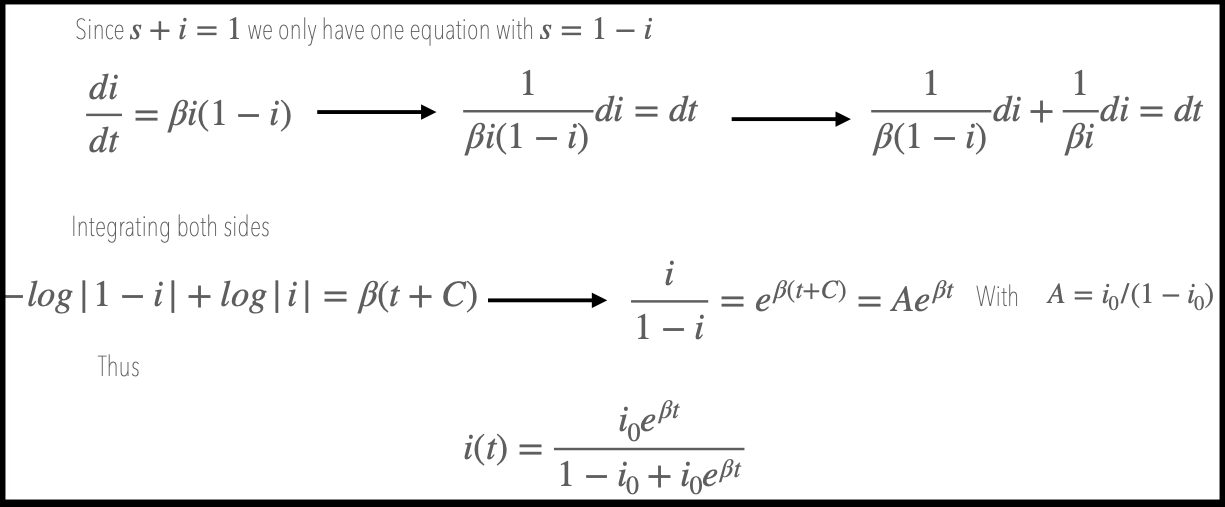
\includegraphics[width=0.9\textwidth]{../lessons/image/03/1.png}
% \caption{\label{fig:3_1} Calculation of the analitic solution for the SI model.}
% \end{figure}
The result is:
\begin{equation}
  i(t) = \frac{i_0 e^{\beta t} }{1-i_0 + i_0 e^{\beta t} }
\end{equation}
which is a sigmoid function (Fig. \ref{fig:3_2}) that always saturates at 1. One should note that after the first part, where the growth is actually exponential \footnote{It is the one we have seen in the media for COVID-19.}, then at a certain point the slope starts to decrease. The reason for this is that the contribution given by the term $s i$, namely the probability of funding new susceptible people, decrease. Finally, we saturates at 1 after some. As can be clearly seen from Fig. \ref{fig:3_2}, it is the value of $\beta$ that drives the spreading. By increasing it, we obtain a faster exponential growth.
This actually was the simplest model one can think of.

\begin{figure}[h!]
\centering
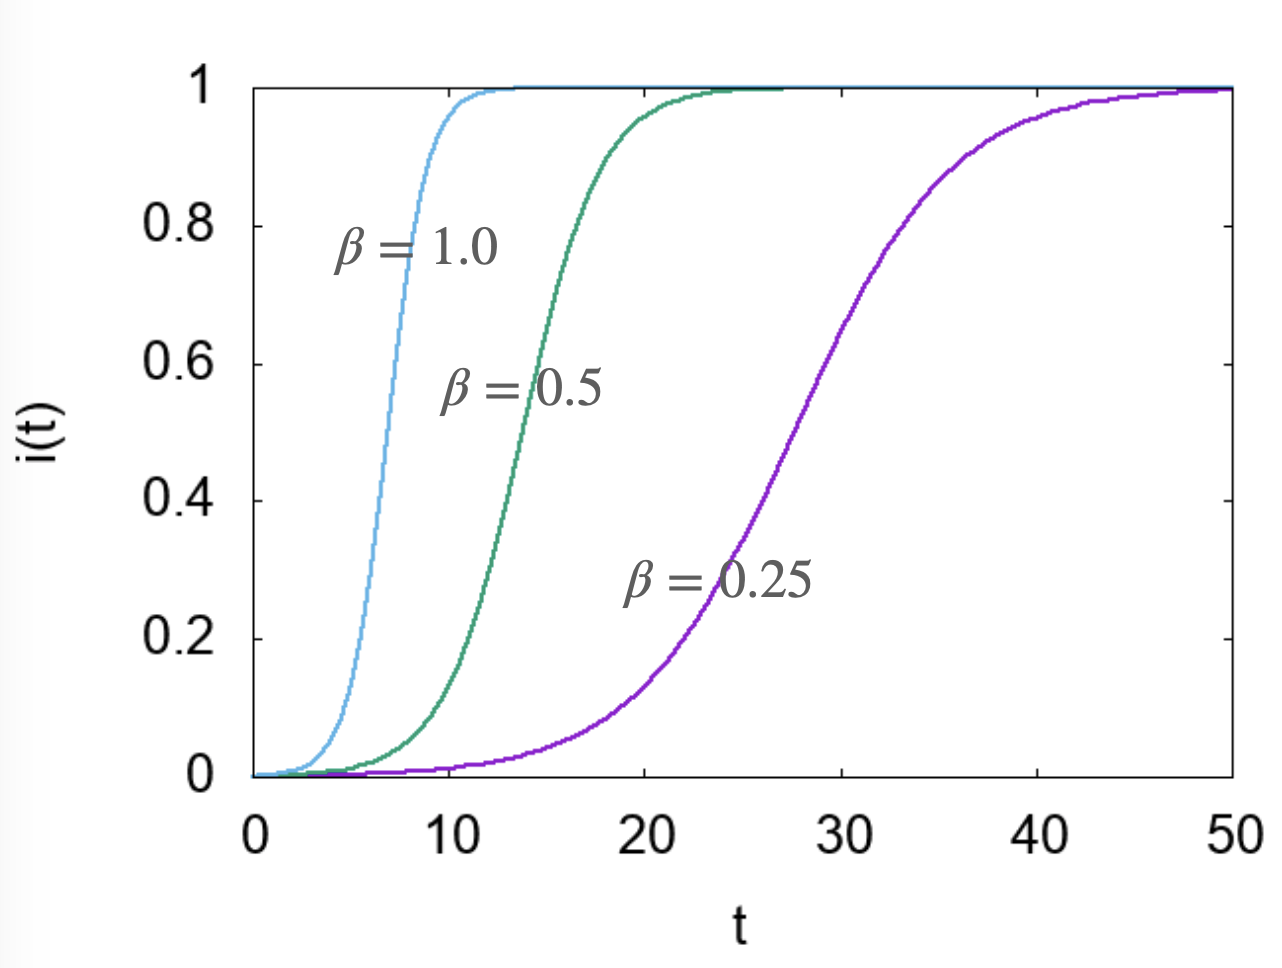
\includegraphics[width=0.7\textwidth]{../lessons/image/03/2.png}
\caption{\label{fig:3_2} Plot of the solution of the SI model for different \( \beta  \).}
\end{figure}

\begin{remark}
In the course we are going to use capital letter for integer numbers, while small letters refer to densities.
\end{remark}

\subsection{SIS model}
Now, let us introduce a slightly more complicated model, that is the \textbf{SIS} model, where compartments are \textbf{S}\textit{usceptible}, \textbf{I}\textit{nfected}, \textbf{S}\textit{usceptible}. Transitions now are two:
\begin{equation}
\begin{split}
  S + I &\overset{\beta }{\rightarrow } I + I \\
  I &\overset{\mu }{\rightarrow } S
\end{split}
\end{equation}
where the first transition is mediated by $I$, that is to say we need to encounter another infected to contract the disease, while the second one occurs \textbf{spontaneously} according to the rate $\mu$.

This model is used for diseases that do not confer immunity. When we use the expression \textbf{endemic state} it means that the disease keeps on circulating in the population for very large times.

The most important feature about this model is that it is the simplest one where \textbf{dynamical equilibrium} can be reached. Therefore an individual may recover from the disease, but he does not get immunity. Indeed there are always people infected that can propagate the disease. The $ \mu  $ is the \textbf{recovery rate} which determines the \textit{time-scale of the infection}. Dividing \( \beta  \) by \( \mu  \) you can \textbf{rescale} all the \textbf{dynamics}.
The \textbf{equations} are exactly the same as before, except for a term:
\begin{equation}
\begin{split}
  \dv{s}{t} &= - \beta \expval{k} si + \mathcolorbox{green!20}{\mu i}  \\
  \dv{i}{t} &= \beta \expval{k} si - \mathcolorbox{green!20}{\mu i}
\end{split}
\end{equation}
and in addition can solved in the very same way we previously did.

Also, the shape of the \textbf{solution} is a sigmoid as before:
\begin{equation}
  i(t) = i_0 \frac{(\beta - \mu ) e^{(\beta - \mu )t} }{(\beta - \mu)  + \beta i_0 (e^{(\beta - \mu )t} - 1) }
\end{equation}
By plotting it, one should note that despite the same form, we do not saturate at 1, but at $ \frac{\beta - \mu }{\beta } $. Hence, as we said, we have some sort of \textbf{dynamical equilibrium}: the number of new infected is more or less the same of the new recovered people at each moment. The density $i(t)$ will therefore fluctuate around this value $\frac{\beta - \mu }{\beta }$ and, by enlarging \( \mu  \), we can obtain larger fluctuations (Fig. \ref{fig:3_3}).
\begin{figure}[h!]
\centering
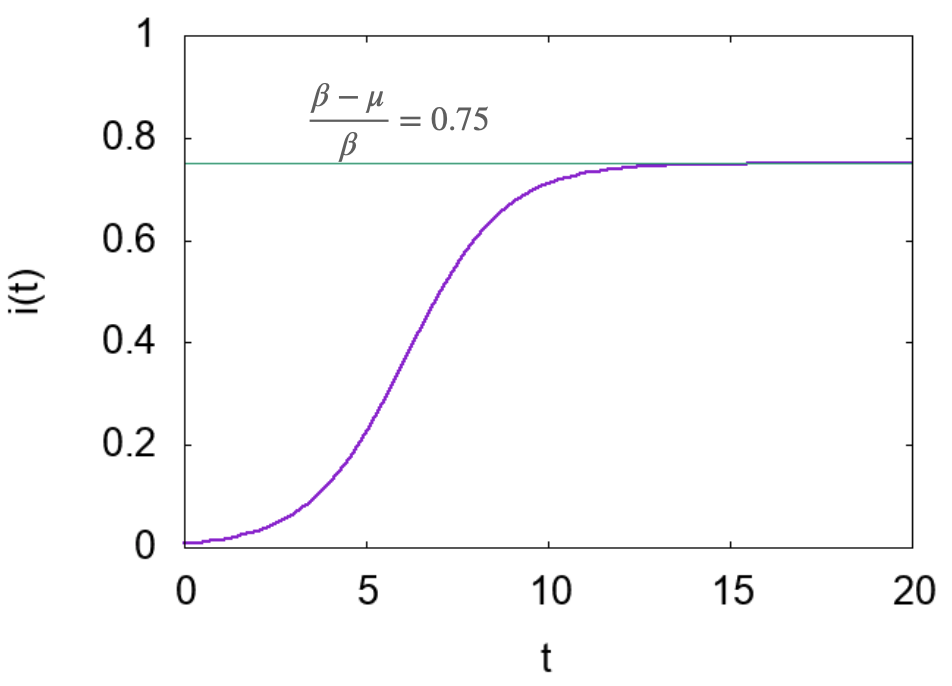
\includegraphics[width=0.7\textwidth]{../lessons/image/03/3.png}
\caption{\label{fig:3_3} Plot of the solution of the SIS model.}
\end{figure}

It can be instructive to study what happens according to this model at the \textbf{transient}. At the beginning, one can assume that almost the entire population is composed by susceptible  people ($ s \sim 1 $), while the number of infected is very small ($ i \ll 1 $).
Hence, the differential equations can be rewritten as following:
\begin{equation*}
  \dv{i}{t} = \beta \expval{k} s i - \mu i \sim \beta \expval{k} i - \mu i \rightarrow i(t) \sim i_0 e^{(\beta \expval{k} - \mu  )t}
\end{equation*}
One should note that if \( \beta \expval{k} < \mu   \) there is no spreading at this point anymore, while, if \( \beta \expval{k} > \mu   \) the exponent becomes positive and from this follows the exponential growth at the beginning (Fig. \ref{fig:3_4}).

\begin{figure}[h!]
\centering
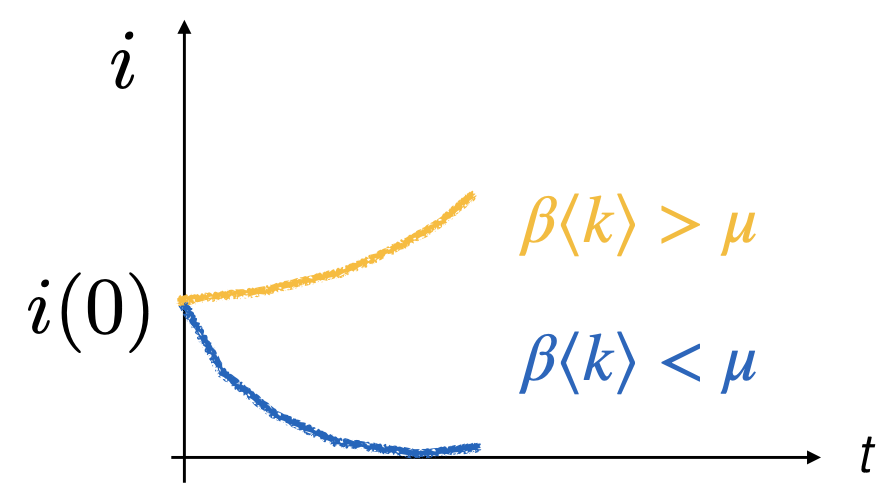
\includegraphics[width=0.6\textwidth]{../lessons/image/03/4.png}
\caption{\label{fig:3_4} Initial transient for the SIS model.}
\end{figure}

One very important thing is that considering the \textbf{steady state} we can have two possible behaviors:
\begin{equation*}
  \dv{i}{t} = 0 \rightarrow  \begin{cases}
   i=0 & \beta \expval{k} < \mu  \\
   i>0 & \beta \expval{k} > \mu
  \end{cases}
\end{equation*}
and we have that:
\begin{equation}
  i>0 \iff \beta > \beta_c = \frac{\mu }{ \expval{k} }
\end{equation}
where $\beta_c$ is known as the \textbf{epidemic threshold}. This tells us whether the disease is going to spread.

In addition the epidemic threshold is the minimum value of the infection probability for which the disease survives. This is what in physics is called a \textbf{second order phase transition} (Fig. \ref{fig:3_5}). In this case the \textbf{critical exponents} are the same of the Ising model, since they belong to the same class of universality. $\beta_c$ is one of the most important quantities we are going to study.

\begin{figure}[h!]
\centering
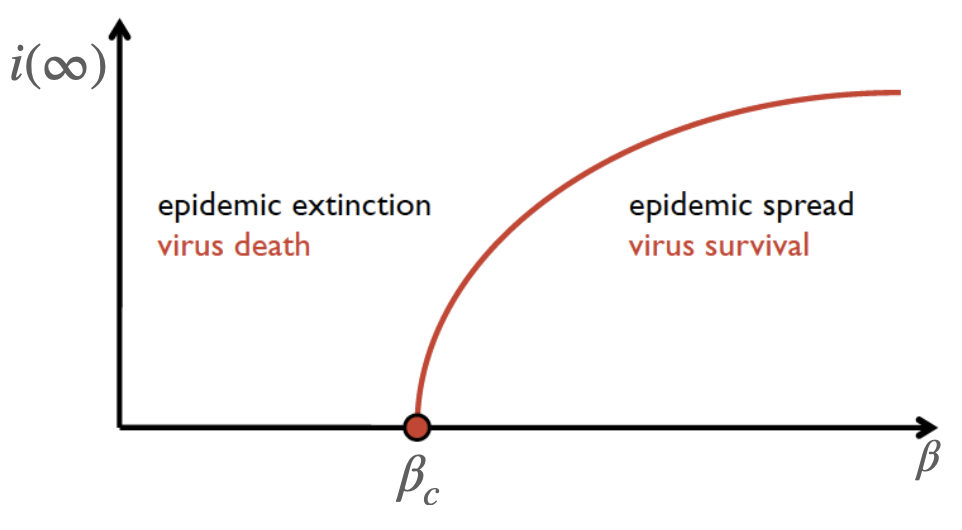
\includegraphics[width=0.7\textwidth]{../lessons/image/03/5.png}
\caption{\label{fig:3_5} Epidemic diagram.}
\end{figure}

One may ask what is the relation between \( R_0 \) and the epidemic threshold. Obviously, they are strongly correlated. We actually say that given a \textbf{critical value}, below it we have no spreading, while above we have a fraction of infected people.

We refer to these two different cases as it follows: if our $\beta < \beta_c$, then we end up in the so called \textbf{epidemic extinction} and the virus, in the long run, will not be present any more. On the other hand, if $\beta > \beta_c$, the virus is going to be present in the population and therefore survives. This is the so called $\textbf{endemic state}$. Behavior around the critical point might be of our interest and can be studied using Statistical mechanics formalism and/or numerical simulations. 

The epidemic threshold is given by the condition under which we observe the spreading. Mathematically, given a specific model, its critical version will return the values of the parameters for which $ R_0 = 1 $. If we are slightly above this threshold, we need a minimum of infected people and the disease is going to spread. Considering for instance the case of the SIS model:
\begin{equation}
  R_0 = \frac{\beta \expval{k} }{\mu } = 1
\end{equation}


\subsection{SIR model}
We now discuss the so called $SIR$ model, whose compartments are \textbf{S}\textit{usceptible}, \textbf{I}\textit{nfected} and \textbf{R}\textit{ecovered}. The idea behind is the same one of the SIS, but we are now adding a new state which accounts for long lasting immunity (\textbf{R}). Hence, once a person has got the disease and has recovered, he obtains a long \textbf{immunity}. Recall that, since we assumed that the population is closed, its density is still fixed to 1.

The transitions for this model are:
\begin{equation}
\begin{split}
  S + I &\overset{\beta }{\rightarrow } I + I  \\
  I &\overset{\mu }{\rightarrow } R
\end{split}
\end{equation}
and one should note that we cannot have any endemic state. For large times all individuals will have been infected, and recovered, so the disease will be spreading no more.

The differential equations that describe this model are:
\begin{equation}
\begin{split}
  \dv{s}{t} &= - \beta \expval{k} si  \\
  \dv{i}{t} &= \overbrace{\beta \expval{k} si}^{\text{New infections}}  - \overbrace{\mu i}^{\text{Recovery}} \\
  \dv{r}{t} &= \mu i
\end{split}
\end{equation}

\begin{figure}[h!]
\centering
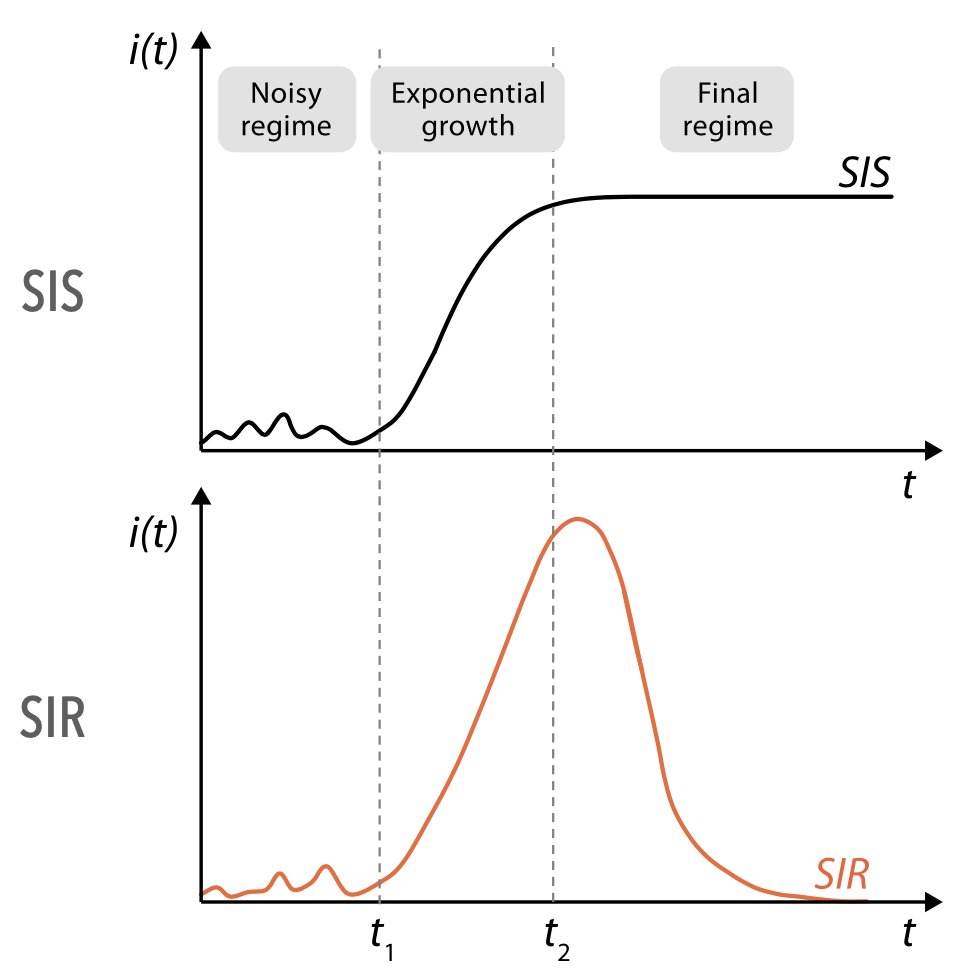
\includegraphics[width=0.6\textwidth]{../lessons/image/03/6.png}
\caption{\label{fig:3_6} Epidemic regimes.}
\end{figure}

This is actually a good point to introduce the \textbf{different regimes} we may encounter during a spreading, which are represented in Fig. \ref{fig:3_6} for the SIS and SIR models.

Initially, at the beginning of each spreading, we see the so called \textbf{noisy phase} where numbers are too small to cause a large spreading. Here we can observe only some sort of stochastic fluctuations. In many cases, we can end up without any spreading: this may happen if we assume that some nodes are much more linked than others (the so called \textit{super spreaders}), and we are able to recognize and stop them before they can infect anyone\footnote{the assumption is one of the basis for \textbf{heterogeneous} mean field models. We will discuss them later in the course.}. If it is not the case, the disease starts spreading according to the characteristic \textbf{exponential growth}. Later, the slope slows down until we reach the \textbf{steady state}: for the SIS the disease keeps circulating among the individuals \textit{(endemic state)}, while for the SIR it disappears \textit{(absorbing state)}.

In order to compute the \textbf{epidemic threshold} for the SIR model, the path to follow is the same as before. In particular, we assume that, at the starting point, $ r \ll 1 $ so that:
\begin{equation*}
  \dv{i}{t} = \beta \expval{k} s i - \mu i \sim \beta \expval{k} i - \mu i \rightarrow i(t) \sim i_0 e^{(\beta \expval{k} - \mu  )t}
\end{equation*}
and the result we find is again:
\begin{equation}
  \beta > \beta _c = \frac{\mu }{\expval{k} }
\end{equation}

Since we are able to obtain an analytic expression for S and I in this SIR model, we want to study what is the behavior for large times ($ t = \infty$ ). One obtains that:
\begin{equation*}
  \dv{s}{r} = \frac{- \beta  \expval{k}  s}{\mu }
\end{equation*}
Assuming moreover that \( r_0 = 0  \) and integrating the above expression wrt \( r \), we obtain:
\begin{equation*}
  s(t) = s_0 e^{-r(t) \frac{\beta \expval{k} }{\mu }}
\end{equation*}
As already said, we cannot find an analytical solution, but we can study the \textbf{behavior for large times} by making some approximations. At \( t=\infty  \), it holds that \( i (\infty ) = 0 \), thus \( s(\infty ) = 1 - r(\infty ) \) because of the closed population assumption:
\begin{equation*}
  1 - r(\infty ) - s_0 e^{-r(\infty ) \overbrace{\frac{\beta \expval{k} }{\mu }}^{R_0}} = 0
\end{equation*}
This is a transcendental equation that cannot be solved analytically, but still gives important hints on the behavior of the disease.\\
One may note that \( R_0 = \beta \expval{k} / \mu   \), and this should make us understand why it is \( R_0 \) that drives the exponential growth of the disease, being it proportional to $\beta \expval{k}$. Moreover, the initial fraction of susceptible people ($s_0$) plays a role in shaping the final fraction of recovered. In particular, if \( s_0 \ll 1 \), the disease cannot spread. This is how \textbf{herd immunity} can be obtained.


\section{Extensions of the SIR model}
We want now to modify the SIR to take into account some more features we want to implement our model with.

\subsection{SIR with Demography}
So far we have assumed that the population was totally closed, and so densities always sum up to 1. This is actually unrealistic, so our next step will be to \textbf{drop} the \textbf{closed population} assumptions: we will now introduce births and deaths. This reasoning is justified from what we observe in real world: considering the demography, we note as every year there are new children that are infected by diseases such as Measles and Chickenpox. Anyway, we do not expect that they will die out over weeks, but still it tells us that newborns increase the populations to the susceptible compartment.

The simplest assumption we can make is: similar to the infectious period, individuals can have a \textbf{lifespan}, denoted as \( 1/\alpha  \) years$^{-1}$. Note as in this approximations lifespan is much greater than the infectious period, so deaths are not due to the disease. In this way we assume that \( \alpha  \) is the death rate, common to all classes. Moreover, \( \alpha  \) is also the crude birth rate, and in addition we assume that births occur only for susceptible individuals and therefore increase its density.

In order to keep the population constant, we need to assume:
\begin{equation}
  \dv{s}{t} + \dv{i}{t} + \dv{r}{t} = 0
\end{equation}

Our equations become then:
\begin{equation}
\begin{split}
  \dv{s}{t} &= \alpha - \beta s i - \alpha s  \\
  \dv{i}{t} &= \beta s i - \mu i - \alpha i \\
  \dv{r}{t} &= \mu i - \alpha r
\end{split}
\end{equation}
where the \textbf{infectious period} is:
\begin{equation}
  \tau = \frac{1}{\alpha + \mu }
\end{equation}
on average, individuals spend less time infected because some of them may die while infected. However, it is a small change compared to before, since lifespan is much greater than the infectious period.

Also, \( \mathbf{R_0} \) is reduced due to mortality:
\begin{equation}
  R_0 = \frac{\beta }{\alpha + \mu }
\end{equation}

We want now to study the \textbf{equilibrium points} of the dynamic for this model. Assuming:
\begin{equation*}
  \dv{s}{t} = \dv{i}{t} = \dv{r}{t} = 0
\end{equation*}
we want to find the \textbf{equilibrium values}  \( s^* \), \( i^* \) and \( r^* \).
It holds that, at equilibrium:
\begin{equation*}
  \dv{i}{t} = 0 = \beta s i - \mu i - \alpha i \quad \rightarrow   \beta s^* i^* - (\mu + \alpha ) i^* = 0
\end{equation*}
and, collecting $i^*$, we obtain the following equation:
\begin{equation}
  i^* \qty[\beta s^* - (\mu + \alpha )] = 0
\end{equation}
which is not differential anymore.

There are two different solutions for this equation: the one for which \( i^* = 0 \) (\textbf{disease free state}) and the one for \( s^* = \frac{\alpha + \mu }{\beta } = \frac{1}{R_0} \), which is the \textbf{endemic state}. Here, the most important result is that the \textbf{SIR} model \textbf{with demography} can actually \textbf{show} an \textbf{endemic state}.

Replacing \( s^* = \frac{1}{R_0} \) in \( \dv{s}{t} = \alpha - \beta s i - \alpha s  \), we obtain:
\begin{equation*}
  i^* = \frac{\alpha R_0 }{\mu } \qty(1 - \frac{1}{R_0}) = \frac{\alpha }{\beta } (R_0 -1)
\end{equation*}
Finally, the three \textbf{equilibrium values} $(s^*, i^*, r^*)$ for the fraction of infected, susceptible and recovered in the endemic state are:
\begin{equation}
  (s^*, i^*, r^*) = \qty( \frac{1}{R_0}, \frac{\alpha }{\beta } (R_0 -1 ), 1- \frac{1}{R_0} - \frac{\alpha }{\beta } (R_0-1))
\end{equation}
Keep in mind that this solution exists only if \( R_0>1 \) and we obtained the equation for $r*$ by reverting the formula $s^* +  i^* + r^* = 1$. Moreover, via linear stability analysis, it can be demonstrated that this equilibrium is stable and is reached through damped oscillations.
\end{document}
